\documentclass[../paper.tex]{subfiles}

% Document
\begin{document}

    ClimaX is the first foundation model designed to perform a wide variety of weather and climate modeling tasks.
    For weather, these tasks include standard forecasting tasks of relevant weather variables like temperature,
    humidity, etc.
    with various lead-times at various resolutions, both globally and regionally.
    For climate, ClimaX can help to make better long-term projections,
    or to downscale lower resolution model outputs to higher resolutions.
    At its core, ClimaX is a multidimensional image-to-image translation architecture based on Vision Transformers
    (ViT).\\
    ViT-based architectures are especially well suited for modeling weather and climate phenomena
    since they naturally tokenize the spatial nature of multiscale data akin to different spatial-temporal inputs.
    Additionally,
    they offer the opportunity to extend tokenization towards a wide range of multichannel features.\cite{d1}
    \subsubsection{Results highlights}
        Forecasting the future values of key weather variables at different temporal horizons is critical
        to ensuring the safety of communities and infrastructure around the world.\\
        ERA5 is the latest climate reanalysis produced by ECMWF,
        providing hourly data on many atmospheric,
        land-surface and sea-state parameters together with estimates of uncertainty.\cite{d2} \\
        ERA5 reanalysis data from the ECMWF underlies as the key source of data for training
        and evaluating machine learning models on this task with performance of Operation
        IFS being the current state-of-the art numerical weather prediction baseline.\\
        ClimaX when fine-tuned on the same ERA5 data,
        even at medium resolutions 1.40625\textdegree already performs comparably,
        if not better than IFS on short and medium-range predictions,
        while being substantially better at longer horizon predictions.\cite{d1}
        \begin{figure}[htbp]
        \centerline{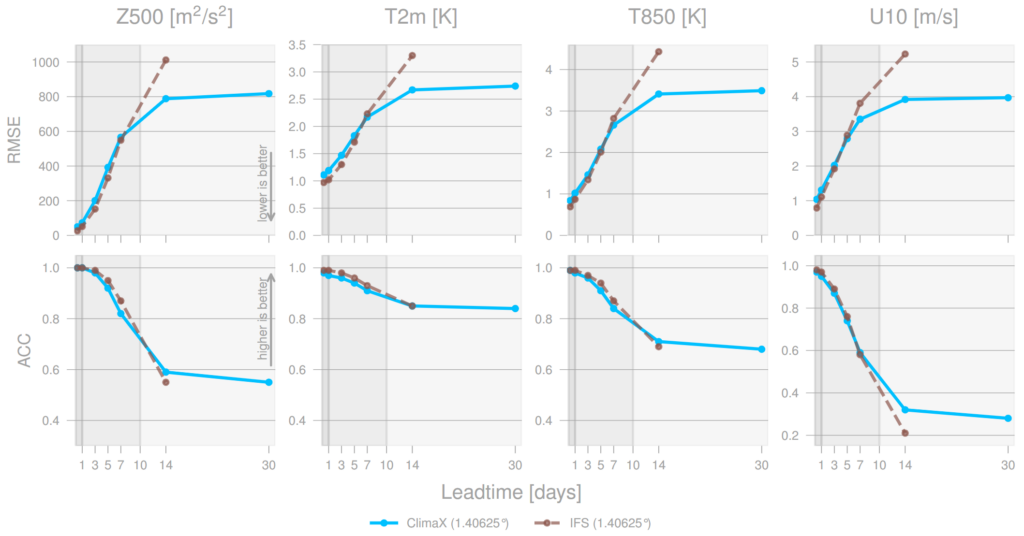
\includegraphics[width=0.5\textwidth]{/C:/Users/oterk/Desktop/University/Ba3INF/Paper-bachelor-proof/src/photos/climax_ifs}}
        \caption{ClimaX vs IFS on global forecasting of key weather variables at different lead time horizons}
        \label{fig:climax-vs-ifs}
        \end{figure}

        In the graphs above,
        we compare the performance of ClimaX vs IFS on global forecasting of key weather variables at different lead time horizons:
        \begin{itemize}
            \item Temperature T2M (2m above ground)
            \item Temperature T850 (850hPa)
            \item Wind speed U10M (10m above ground)
            \item Geo-potential height Z500 (500hPa)
        \end{itemize}
        The graphs on the first row show the RMSE (root mean squared error) of the predictions,
        while the graphs on the second row show the ACC (accuracy) of the predictions.
        The x-axis shows the lead time in days.
        As we can see, for example, on the Z500 graph, both models start at \%accuracy 100 and 0 RMSE.\\
        As the lead time increases, the accuracy of both models decreases, and the error increases.
        What a decrease in accuracy means is that the model is less confident in its predictions.\\
        The lower the accuracy, the more uncertain the model is and the higher the error.
        A higher error means that the model is less accurate and less trustworthy.
        \\\\
        But as we can see, ClimaX performs somewhat comparably to IFS on short and medium-range predictions,
        while being substantially better at longer horizon predictions (in most of these graphs, 14 days and above).
    \subsubsection{Motivation}
        ClimaX provides a variety of different spatial-temporal resolutions and input channels,
        which can be used for a wide variety of weather and climate modeling tasks.
        Being benchmarked against other state-of-the-art models, it holds its own and even outperforms them in some cases.


\end{document}